%% 
%% Copyright 2007-2020 Elsevier Ltd
%% 
%\documentclass[preprint,12pt,authoryear]{elsarticle}

%% Use the option review to obtain double line spacing
%\documentclass[preprint,review,12pt]{elsarticle}

% \documentclass[times, review, 10pt]{elsarticle}
\documentclass[5p,times]{elsarticle}


%% The amssymb package provides various useful mathematical symbols
\usepackage{amssymb}
%% The amsthm package provides extended theorem environments
% \usepackage{amsthm}
\usepackage{amsmath}
\usepackage{amsthm}
\usepackage{graphicx}
\usepackage{mathtools}
\usepackage{subcaption}
\usepackage{caption}
\usepackage[linesnumbered,ruled,vlined]{algorithm2e}
\usepackage{booktabs}


\usepackage{lineno}
\usepackage[table,xcdraw]{xcolor}

% Custom imports...
\usepackage{xcolor}
\usepackage{hyperref}
\usepackage{xspace}
\usepackage{comment}
\usepackage{multirow}
\usepackage{multicol}
\usepackage{arydshln}
\usepackage{float}
\usepackage{bbm}
\usepackage{tcolorbox}
\usepackage{booktabs}
% \usepackage{fdsymbol}

\usepackage{caption}
\captionsetup{justification=raggedright}

\journal{Pattern Recognition}

%our macro:
\newcommand{\diff}[2]{\frac{\partial #1}{\partial #2}}
\newcommand{\vct}[1]{\ensuremath{\boldsymbol{#1}}}
% \newcommand{\vct}[1]{\ensuremath{\boldsymbol{\mathbf{#1}}}}

\newcommand{\mat}[1]{\ensuremath{\mathbf{#1}}}
\newcommand{\set}[1]{\ensuremath{\mathcal{#1}}}
\newcommand{\con}[1]{\ensuremath{\mathsf{#1}}}
\newcommand{\tsum}{\ensuremath{\textstyle \sum}}
\newcommand{\T}{\ensuremath{\top}}

\newcommand{\soa}{state-of-the-art\xspace}
\newcommand{\mycomment}[1]{\textcolor{red}{#1}}
\newcommand{\ind}[1]{\ensuremath{\mathbbm 1_{#1}}}
\DeclareMathOperator*{\argmin}{arg\,min}
\DeclareMathOperator*{\argmax}{arg\,max}
\DeclareMathOperator*{\minimize}{minimize}
\DeclareMathOperator*{\maximize}{maximize}
\DeclareMathOperator*{\subjectto}{subject~to}
\DeclareMathOperator*{\st}{s.t.}
\newcommand{\erf}{\text{erf}}
\newcommand{\sign}{\text{sign}}
\newcommand{\bmat}[1]{\begin{bmatrix}#1\end{bmatrix}}
%\newcommand{\myparagraph}[1]{\medskip \noindent \textbf{#1}}
\newcommand{\myparagraph}[1]{\noindent \textbf{#1}.}
%\newcommand{\mysubparagraph}[1]{\smallskip \noindent \textit{#1}}
\newcommand{\mysubparagraph}[1]{\noindent \textit{#1}}
\newcommand{\mysubpar}[1]{\smallskip \noindent \textit{#1}}
\newcommand{\mylist}[1]{\noindent \textit{#1}}


% Add a period to the end of an abbreviation unless there's one
% already, then \xspace.
\makeatletter
\DeclareRobustCommand\onedot{\futurelet\@let@token\@onedot}
\def\@onedot{\ifx\@let@token.\else.\null\fi\xspace}

\newcommand{\ie}{i.e.,\xspace}
\newcommand{\eg}{e.g.,\xspace}
\newcommand{\aka}{a.k.a.\xspace}
\newcommand{\wrt}{w.r.t.\xspace}

\newcommand{\quotes}[1]{``{\textit{#1}}''\xspace}
\newcommand{\doublequotes}[1]{``{#1}''\xspace}
\newcommand{\singlequotes}[1]{`{#1}'\xspace}

\newcommand{\ellzero}{$\ell_0$\xspace}
\newcommand{\ellone}{$\ell_1$\xspace}
\newcommand{\elltwo}{$\ell_2$\xspace}
\newcommand{\ellinf}{$\ell_{\infty}$\xspace}

\newcommand{\daniele}[1]{\textcolor{red}{Daniele: #1}}
\newcommand{\battista}[1]{\textcolor{orange}{Battista: #1}}
\newcommand{\maura}[1]{\textcolor{cyan}{Maura: #1}}
\newcommand{\lea}[1]{\textcolor{violet}{Lea: #1}}

\newcommand{\yes}{\textcolor{Green}{\ding{51}}}%
\newcommand{\no}{\textcolor{BrickRed}{\ding{55}}}%

%%%%%%%%%%%%%%%%%%%%%%%%%%%%%%%%%%%%%%%%%%%%%%%%%%%%%%%%
% General Math
%%%%%%%%%%%%%%%%%%%%%%%%%%%%%%%%%%%%%%%%%%%%%%%%%%%%%%%%
% Losses
\newcommand{\Loss}{\ensuremath{\mathcal{L}}\xspace}
\newcommand{\loss}{\ensuremath{\ell}\xspace}
\newcommand{\celoss}{\ell_{CE}}
\newcommand{\distloss}{\ell_{D}}

%Notation
\newcommand{\numsamples}{\ensuremath{n}\xspace}
\newcommand{\sampleindex}{\ensuremath{i}\xspace}
\newcommand{\numfeatures}{\ensuremath{d}\xspace}
\newcommand{\featureindex}{\ensuremath{j}\xspace}
\newcommand{\numclasses}{\ensuremath{c}\xspace}
\newcommand{\classindex}{\ensuremath{k}\xspace}

\newcommand{\vgrad}{\ensuremath{\vct{g}}\xspace}
\newcommand{\grad}[2]{\ensuremath{\nabla_{#2}{#1}}\xspace}
\newcommand{\prediction}[1]{\ensuremath{\operatorname{argmax}(#1(\vct x))}}
\newcommand{\predictionsample}[1]{\ensuremath{\operatorname{argmax}(#1(\vct x_i))}}

\newcommand{\f}{\ensuremath{f}\xspace}
\newcommand{\vparams}{\ensuremath{\vct \theta}\xspace}
\newcommand{\ParamSpace}{\ensuremath{\Theta}\xspace}

\newcommand{\x}{\ensuremath{\vct{x}}\xspace}
\newcommand{\X}{\ensuremath{\set{X}}\xspace}
\newcommand{\Y}{\ensuremath{\set{Y}}\xspace}
\newcommand{\Ball}{\ensuremath{\mathcal{B}}\xspace}

\newcommand{\ypred}{\hat{y}\xspace}

% Datasets
\newcommand{\ds}{\ensuremath{\mathcal{D}}} % generic dataset
\newcommand{\tr}{\ensuremath{\set D}\xspace}
\newcommand{\ts}{\ensuremath{\set T}\xspace}
\newcommand{\val}{\ensuremath{\set V}\xspace}


\renewcommand{\sectionautorefname}{Sect.}
\renewcommand{\subsectionautorefname}{Sect.}
\renewcommand{\subsubsectionautorefname}{Sect.}
\renewcommand{\equationautorefname}{Eq.}
\renewcommand{\figureautorefname}{Fig.}


\begin{document}
\setcitestyle{square} %[GS] Questo mette le parentesi quadre, fare ultimo check sulla submission che tipo di parentesi vogliono

\begin{frontmatter}

%\title{Buffer-free Incremental Learning in Open World}
\title{Continual Learning Security Survey}

%% use optional labels to link authors explicitly to addresses:
\author[unica,uniroma]{Daniele Ghiani}
\ead{daniele.ghiani@unica.it}

\author[unica]{Ambra Demontis}
\ead{ambra.demontis@unica.it}

\author[unica]{Daniele Angioni}
% \ead{daniele.angioni@unica.it}

\author[unica]{Maura Pintor}

\author[unipi]{Antonio Carta}
%\ead{ambra.demontis@unica.it}

\author[unipi]{Davide Bacciu}
%\ead{ambra.demontis@unica.it}

\author[unica]{Battista Biggio}
% \ead{battista.biggio@unica.it}

\affiliation[unica]{organization={DIEE, University of Cagliari}, 
            addressline={Via Marengo 2}, 
            city={Cagliari},
            postcode={09100}, 
            country={Italy}}

\affiliation[uniroma]{organization={DIAG, Sapienza University of Rome}, 
            addressline={Via Ariosto 25}, 
            city={Roma},
            postcode={00185}, 
            country={Italy}}
            

\affiliation[unipi]{organization={DIEE, University of Pisa}, 
            addressline={Lungarno Antonio Pacinotti, 43}, 
            city={Pisa},
            postcode={56126}, 
            country={Italy}}

\begin{abstract}
% Context (1 sentence)
% Gap (CL changes threat model → not covered)
% Contribution (taxonomy + insights)
% Key insight (temporal persistence / delayed attacks / memory as attack surface)
% Optional: evaluation/benchmarking perspective
- ML is being deployed in dynamic environments, which makes CL the paradigm of choice
- Security is well-studied in static environments, but the dynamics of CL fundamentally changes the threat model, from both attacker's and defender's perspective.
- In this work, we are the first to survey existing literature on adversarial attacks and defenses in the context of CL
- We provide a renewed threat model, highlighting the unique security challenges that arise when learning sequential tasks without revisiting old data.
- (BONUS) mention experiments?
\end{abstract}
% CL introduces temporal attack surfaces and persistence effects absent in static ML
% Existing AML taxonomies fail to capture these
% We provide:
% unified threat model (temporal-aware)
% taxonomy of attack surfaces (data stream, memory, generator, prompts, init)
% classification of attacks by persistence and activation time
% critical analysis of evaluation flaws
% Key insight: security in CL is dominated by persistence, not just accuracy degradation

\begin{keyword}
%% keywords here, in the form: keyword \sep keyword
continual learning \sep
adversarial machine learning \sep
neural networks.
%% PACS codes here, in the form: \PACS code \sep code
%% MSC codes here, in the form: \MSC code \sep code
%% or \MSC[2008] code \sep code (2000 is the default)
\end{keyword}

\end{frontmatter}

% \linenumbers

\section{Introduction - fine dicembre}
% persistence of malicious patterns
% delayed attacks
\textcolor{red}{TODO}
Contributions:
\begin{itemize}
\item First survey on CL security
\item thorough analysis of attack surfaces brought by the CL setting

\end{itemize}

\section{Continual Learning - fine ottobre}
Basic definitions and notation
\textcolor{red}{brief overview, minimal info to understand the security part}

\begin{itemize}
    \item class, task, domain incremental learning  
    \item metodi (es replay etc) 
    \item metriche
\end{itemize}


\section{Threat Model - fine novembre}

\textcolor{red}{Here we can build backward from Sect 3, depending on what we need to define}


\textcolor{red}{TODO: da adatttare focalizzando tutto su CL}

\subsubsection{Attacker's Goal}
\myparagraph{Security Violation} integrity, availability, privacy.
\myparagraph{Attack Specificity} which samples the attacker is targeting. Sample-specific (targeted) / sample-generic (indiscriminate)
% \myparagraph{\textcolor{red}{Task Specificitiy}} which tasks the attacker is targetting (past tasks, current, or future tasks)
\myparagraph{Error Specificity} which classes are the targets (error-generic / error-specific)

\subsubsection{Attacker's Knowledge} white-box / gray-box / black-box

\subsubsection{Attacker's Capability}
\myparagraph{Influence on Learning Setting}
In Training from scratch and Fine tuning the attacker only controls part of the training data.
In Model training the attacker is the third-party trainer.
\myparagraph{Data Manipulation Constraint} same of static learning (no works on clean label attacks) 


\textcolor{red}{TODO: da integrare su:}

\begin{table*}[t]
\centering
\small
\resizebox{\linewidth}{!}{
\begin{tabular}{llp{5cm}p{5cm}p{5cm}}
\toprule
 &  & \textbf{Integrity} & \textbf{Availability} & \textbf{Confidentiality} \\
\midrule
\multirow{2}{*}{\textbf{Test data}} 
& \textit{Attacks} 
& evasion attack 
& continual sponge (NA) 
& model inversion (for past tasks); membership inference (NA) \\
\cline{2-5}
& \textit{Defenses} 
& Continual AT 
& stateful defenses (NA) 
& continual differential privacy \\
\midrule
\multirow{2}{*}{\textbf{Training data}} 
& \textit{Attacks} 
& persistent backdoor; latent backdoor; targeted forgetting 
& indiscriminate forgetting 
& privacy leakage poisoning \\
\cline{2-5}
& \textit{Defenses} 
& c. robust training, c. data sanitization, model inspection, c. model sanitization, trigger reconstruction
& continual data sanitization 
& NA \\
\bottomrule
\end{tabular}
}
\caption{Summary of attacks and defenses across CL security dimensions.}
\label{tab:security_cl}
\end{table*}

\begin{figure*}[t!]
    \centering
    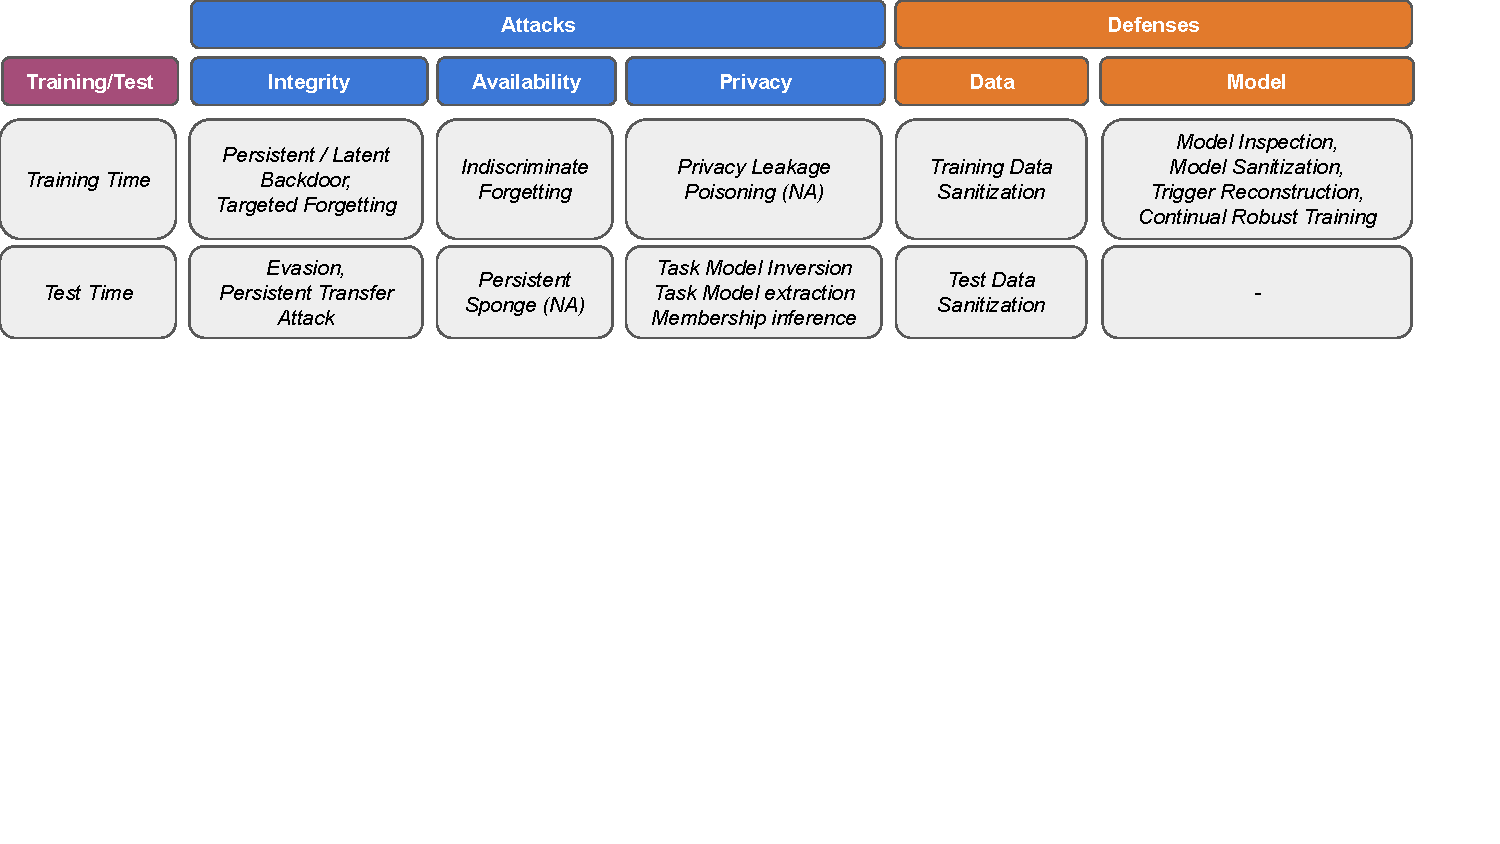
\includegraphics[width=0.99\linewidth]{images/CLSec Slides.pdf}
    \caption{Summary of attacks and defenses across CL security dimensions.}
    \label{fig:temporal_plots_tesseract}
\end{figure*}

\myparagraph{CL Attack Surfaces}
- current task data
- replay memory
- generator (DGR-like methods)
- Model parameters: select stable parameters for longlasting attack effectiveness, attack conditioning during pre-training, prompt-pool

\myparagraph{CL security issues}
\begin{itemize}
\item no access to past data: attacks based on past classes are more difficult
\item incremental learning: risk of erasing important parameters useful for an attack to work (e.g., backdoor triggers)
\item defender cannot monitor performance on past tasks -> high forgetting might be unnoticed
\item stealthiness: attacker should preserve performance on current task (otherwise is a standard attack) \textit{while targeting forgetting}
\item the model used to create the attack might be different to the model on which the attack is executed (e.g., backdoor, transfer attacks, latent backdoor for future tasks)
\end{itemize}

% \myparagraph{Attack Constraint}
% - No access to past data
% - limited control over future tasks (only one paper does that)
% - Partial knowledge of task boundaries
% - stealthiness: performance on current task must be preserved

% \myparagraph{Defense constraints and limitations}
% - CL models, especially memory-free ones, canot easily verify past-task performance as it's unavailable -> attacks are harder to spot
% - CL objective of retaining past knowledge can enhance attack longlasting effect (e.g., backdoor trigger remain effective for multiple tasks)
% - replay memory is a potential attack vector
% - the evaluation becomes more complex, as it must be reiterated for each new task (and possibly the available old samples)



\subsection{Task-aware threat model}
Mismatch between the task being updated and the task being attacked. At step $t$, the learner updates the model using the current task data $\mathcal{D}_t$, yet the adversary may aim to damage one or more past tasks $\mathcal{T}_k$ with $k<t$. This differs from the standard static setting, where the optimized objective and the attacked objective typically coincide.

Formally, let $\theta_{t-1}$ be the model before learning task $\mathcal{T}_t$, and let $\tilde{\mathcal{D}}_t$ denote the manipulated version of the current training data. The continual learner produces
\[
\theta_t = \mathcal{A}(\theta_{t-1}, \tilde{\mathcal{D}}_t, \mathcal{M}_{t-1}),
\]
where $\mathcal{A}$ is the CL update rule and $\mathcal{M}_{t-1}$ denotes any retained summary of the past, such as a replay buffer, a generator, regularization statistics, or prompt-based components. The attacker typically seeks to maximize damage on a target set of past tasks
\[
\mathcal{S}_t \subseteq \{1,\dots,t-1\},
\]
while preserving the apparent correctness of the current update. This can be abstracted as
\[
\max_{\tilde{\mathcal{D}}_t \in \mathcal{B}(\mathcal{D}_t)}
\; \mathcal{L}_{\text{target}}(\theta_t;\mathcal{S}_t)
\quad \text{s.t.} \quad
\mathcal{L}_{\text{curr}}(\theta_t;\mathcal{T}_t) \le \epsilon .
\]

This formulation captures the core asymmetry of CL attacks: the adversary manipulates the current task in order to compromise past knowledge. Depending on the threat model, the target set $\mathcal{S}_t$ may correspond to a single past task, a subset of past tasks, a specific class within a past task, or a persistent trigger-based behavior that should survive subsequent updates. 


\section{Attacks against Continual Learning - fine novembre}
\mycomment{nb: la parte che c'è sotto è solo inference time, training time è commentata}
Main risks: evasion attacks, model inversion.
The attack strategy does not change, 
\textcolor{red}{MA in teoria attaccante non sa quando cambia il modello}
while the defender must be account for different issues.

\subsection{Integrity}

\myparagraph{Evasion attacks in CL}
Here, the way of attacking is the same as the static case.
But the defenses have some complications and require specific care: while CL causes obfuscated gradients, AT causes accelerated forgetting~\cite{Mi-ICCV2025}.
Other works doing AT in CL -> \cite{Khan-IJCNN2022, Chen-TMLR2022, Bai-ICASSP2023}

\textcolor{red}{Attacchi black box diventano complicati se attaccante non sa quando cambia il task.
modelli più stabili, e.g., prompt-based? possono essere più vulnerabili a questo}

\myparagraph{Activating the backdoor in CL}
Similar to evasion attack, backdoored samples can seamlessly evade a classifier. The application does not differ during inference-time attack, but as we will see in next sections, they require several countermeasures at training time in order to work~\cite{Jiang-TDSC2024, Gao-NeuralNetworks2025, Guo-USENIX2025, Nguyen-AAAI2025}.

\subsection{\textcolor{red}{Availability}}
\textcolor{red}{Here we would have sponge attacks but no one have implemented them in CL. DoS Poisoning?}

\subsection{Privacy}
\myparagraph{Model inversion as primary attack vector}
\cite{Du-IJCNN2023} shows how model inversion is necessary to "unlock" poisoning attack, as past data approximations is required to use them.

\myparagraph{Enabling privacy in CL models}
\cite{Hassanpour-IEEEAccess2022} adjust differential-privacy training to be compatible with CL, as in its naive application, the forgetting is too high.


%\section{Training-time CL Security}
%Here is the opposite, plenty of new attack implementations, but lack of defensive strategies. The only one is \cite{Umer-IEEEAccess2024} with a naive approach against backdoor (AT using backdoored samples)


%\subsection{Integrity attacks}
%\myparagraph{Backdoors}
%\cite{Jiang-TDSC2024, Gao-NeuralNetworks2025, Guo-USENIX2025, Nguyen-AAAI2025}
%Main changes: 
%concept of backdoor persistence

%\myparagraph{Targeted poisoning}
%\cite{Umer-IJCNN2021, Li-IJCNN2022, Umer-IJCNN2020}

%\subsection{Availability attacks}
%Main idea: cause global forgetting without influencing the current task
%Necessary condition: attacking past classes requires approximating it with model inversion
%WB: \cite{Han-ICIP2023, Kang-ICML2023, Abbasi-CVPR2024, Umer-IJCNN2020}
%BB: \cite{Perla-WACV2025, Yu-AAAI2024}


\subsection{\textcolor{red}{Privacy}}
\textcolor{red}{No works here}

\subsection{Future Research Directions}

\section{Continual Learning Defenses}
\subsection{Integrity}
\subsection{Privacy}

\subsection{Future Research Directions}

\section{Related work - fine dicembre}
Discuss survey on AML, poisoning and CL
No prior survey on CL security

\subsection{Other synergies between CL and adversarial ML}
\myparagraph{CL for robustness}
Some works use CL concepts to solve robustness-related tasks~\cite{Chou-CW2022, Zhou-CVPR2024, Pham-ECCV2024}, such as modeling new attackers as sequential tasks, or using CL to make a backdoor stronger in a static setting.

\myparagraph{Robustness for CL}
On the opposite, some other works~\cite{Kumari-NeurIPS2022, Wang-ICML2022, Yu-AAAI2025} use adversarial techniques to improve CL clean accuracy and reduce forgetting, e.g., by using AT as a regularizer

\section{Concluding Remarks - fine dicembre}

\section*{Acknowledgments}


\biboptions{sort&compress}
\bibliographystyle{elsarticle-num} 
\bibliography{bibliography}

% \begin{thebibliography}{10}
% \expandafter\ifx\csname url\endcsname\relax
%   \def\url#1{\texttt{#1}}\fi
% \expandafter\ifx\csname urlprefix\endcsname\relax\def\urlprefix{URL }\fi
% \expandafter\ifx\csname href\endcsname\relax
%   \def\href#1#2{#2} \def\path#1{#1}\fi

% \end{thebibliography}


\end{document}
